\documentclass[a4paper,12pt]{article}

% Packages
\usepackage{graphicx}      % For including images
\usepackage{caption}       % Better captions
\usepackage{subcaption}    % Subfigures
\usepackage{geometry}      % Page margins
\usepackage{hyperref}      % Hyperlinks
\usepackage{fancyhdr}      % Header/Footer
\usepackage{amsmath, amssymb} % Math
\usepackage{float}         % Figure positioning


\geometry{margin=1in}
\pagestyle{fancy}
\fancyhead[L]{Machine Learning Final Project}
\fancyhead[R]{\today}
\fancyfoot[C]{\thepage}

% Title
\title{\textbf{Image Classification of MouseCam Animals}}
\author{}
\date{\today}

% Document Start
\begin{document}

\maketitle


\vspace{1cm}

% -----------------------------------------------------
\section{Introduction}
The goal of this project is to develop a robust image classification pipeline for images captured in MouseCams by Dr. John Porter at the University of Virginia. Initially, I aimed to classify all the images using a neural network, but the classifications were extremely unbalanced. For example, about a quarter of the images (8,000 or so) are *Mus musculus*, while species like *Procyon lotor* and *Mus musculus* (both pictured) only have one image each. Additionally, I encountered significant memory issues when attempting to run this analysis. While I tried to get it working on the cluster, I faced challenges in creating a working environment that could generate the plots needed for troubleshooting the data processing. For these reasons, I chose to resize the 5 MB images during preprocessing and include a maximum of 500 images per classification. This resulted in a dataset of 3,216 images to train the model, consisting of the classifications: Bird, Crab, *Glaucomys volans*, Insect, *Microtus pennsylvanicus*, *Mus musculus*, *Orozomys palustris*, *Peromyscus leucopus*, *Procyon lotor*, *Rattus norvegicus*, Snake, *Sorex* sp., and *Sylvilagus*. I also structured the code to easily process more images on a higher-powered computer or to include additional classifications (e.g., Unidentified Rodent, Other, etc.) if desired.


\section{Data Preprocessing}
The images were preprocessed using the following steps:
\begin{enumerate}
    \item Downloading and filtering images. I removed the bottom 100 pixels from the image to take away the bottom information pasted on by the camera. I also removed 150 pixels from each side of the images to take away the sides of the bucket.
    \item Cropping and resizing images to $256 \times 256$ dimensions.
    \item Splitting the dataset into training (80 percent) and testing (20 percent) sets.
\end{enumerate}

The resulting datasets include:
\begin{itemize}
    \item \textbf{Training set}: 80\% of the images.
    \item \textbf{Testing set}: 20\% of the images.
\end{itemize}

\section{Model Training and Selection}

Three models were trained for image classification:

\subsection{Model 1: Simple CNN}
The first model is a simple convolutional neural network (CNN) architecture. It includes a single convolutional layer, a max-pooling layer, and two dense layers.

\begin{verbatim}
model_1 <- keras_model_sequential() %>%
  layer_conv_2d(filters = 32, kernel_size = c(3, 3), activation = 'relu', input_shape = c(256, 256, 3)) %>%
  layer_max_pooling_2d(pool_size = c(2, 2)) %>%
  layer_flatten() %>%
  layer_dense(units = 128, activation = 'relu') %>%
  layer_dense(units = 13, activation = 'softmax')

model_1 %>% compile(
  optimizer = 'adam',
  loss = 'categorical_crossentropy',
  metrics = c('accuracy')
)
\end{verbatim}

\subsection{Model 2: Larger CNN}
The second model adds complexity by including an additional convolutional layer and increasing the number of filters in each layer.

\begin{verbatim}
model_2 <- keras_model_sequential() %>%
  layer_conv_2d(filters = 64, kernel_size = c(3, 3), activation = 'relu', input_shape = c(256, 256, 3)) %>%
  layer_max_pooling_2d(pool_size = c(2, 2)) %>%
  layer_conv_2d(filters = 128, kernel_size = c(3, 3), activation = 'relu') %>%
  layer_max_pooling_2d(pool_size = c(2, 2)) %>%
  layer_flatten() %>%
  layer_dense(units = 256, activation = 'relu') %>%
  layer_dense(units = 13, activation = 'softmax')

model_2 %>% compile(
  optimizer = 'sgd',
  loss = 'categorical_crossentropy',
  metrics = c('accuracy')
)
\end{verbatim}

\subsection{Model 3: CNN with Dropout Layers}
The third model incorporates dropout layers to reduce overfitting, which improved the generalization performance.

\begin{verbatim}
model_3 <- keras_model_sequential() %>%
  layer_conv_2d(filters = 64, kernel_size = c(3, 3), activation = 'relu', input_shape = c(256, 256, 3)) %>%
  layer_max_pooling_2d(pool_size = c(2, 2)) %>%
  layer_dropout(rate = 0.25) %>%
  layer_conv_2d(filters = 128, kernel_size = c(3, 3), activation = 'relu') %>%
  layer_max_pooling_2d(pool_size = c(2, 2)) %>%
  layer_dropout(rate = 0.5) %>%
  layer_flatten() %>%
  layer_dense(units = 512, activation = 'relu') %>%
  layer_dense(units = 13, activation = 'softmax')

model_3 %>% compile(
  optimizer = 'rmsprop',
  loss = 'categorical_crossentropy',
  metrics = c('accuracy')
)
\end{verbatim}


The accuracy plots for each model are shown below:

\subsection{Accuracy Plots}
\begin{figure}[H]
    \centering
    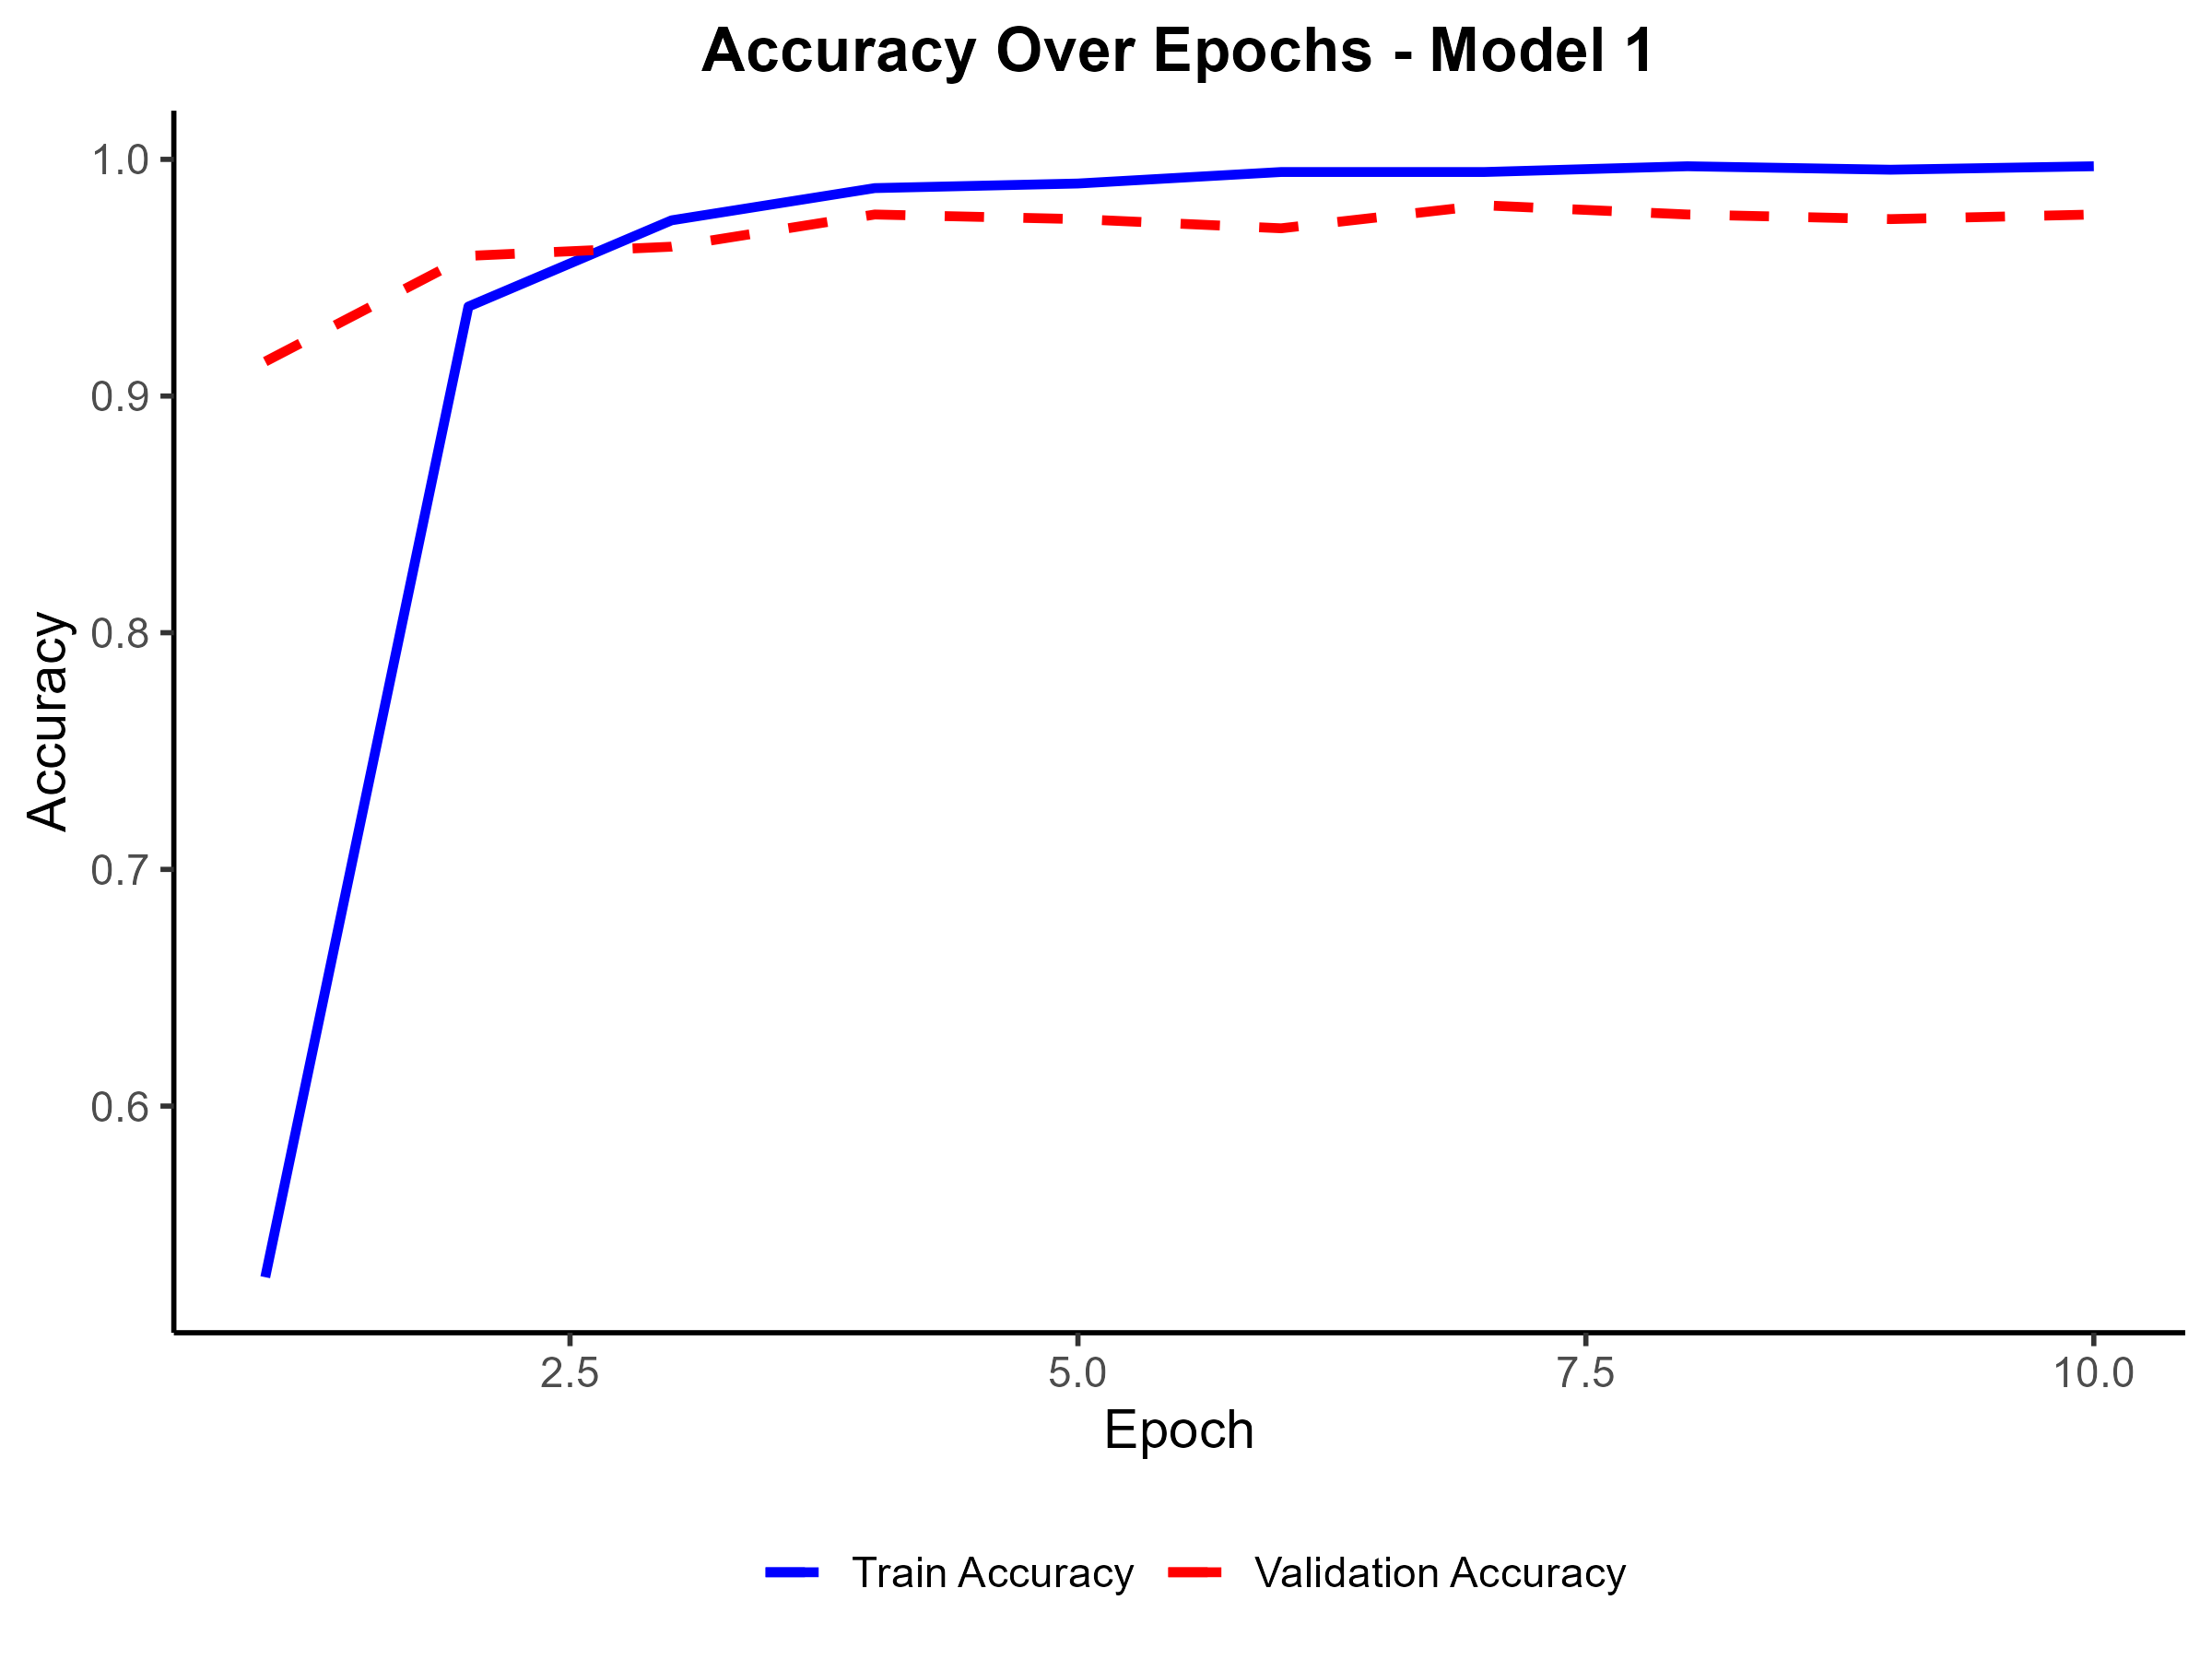
\includegraphics[width=0.8\linewidth]{results/accuracy_plot_model_1.png}
    \caption{Accuracy over epochs - Model 1 (Simple CNN).}
\end{figure}

\begin{figure}[H]
    \centering
    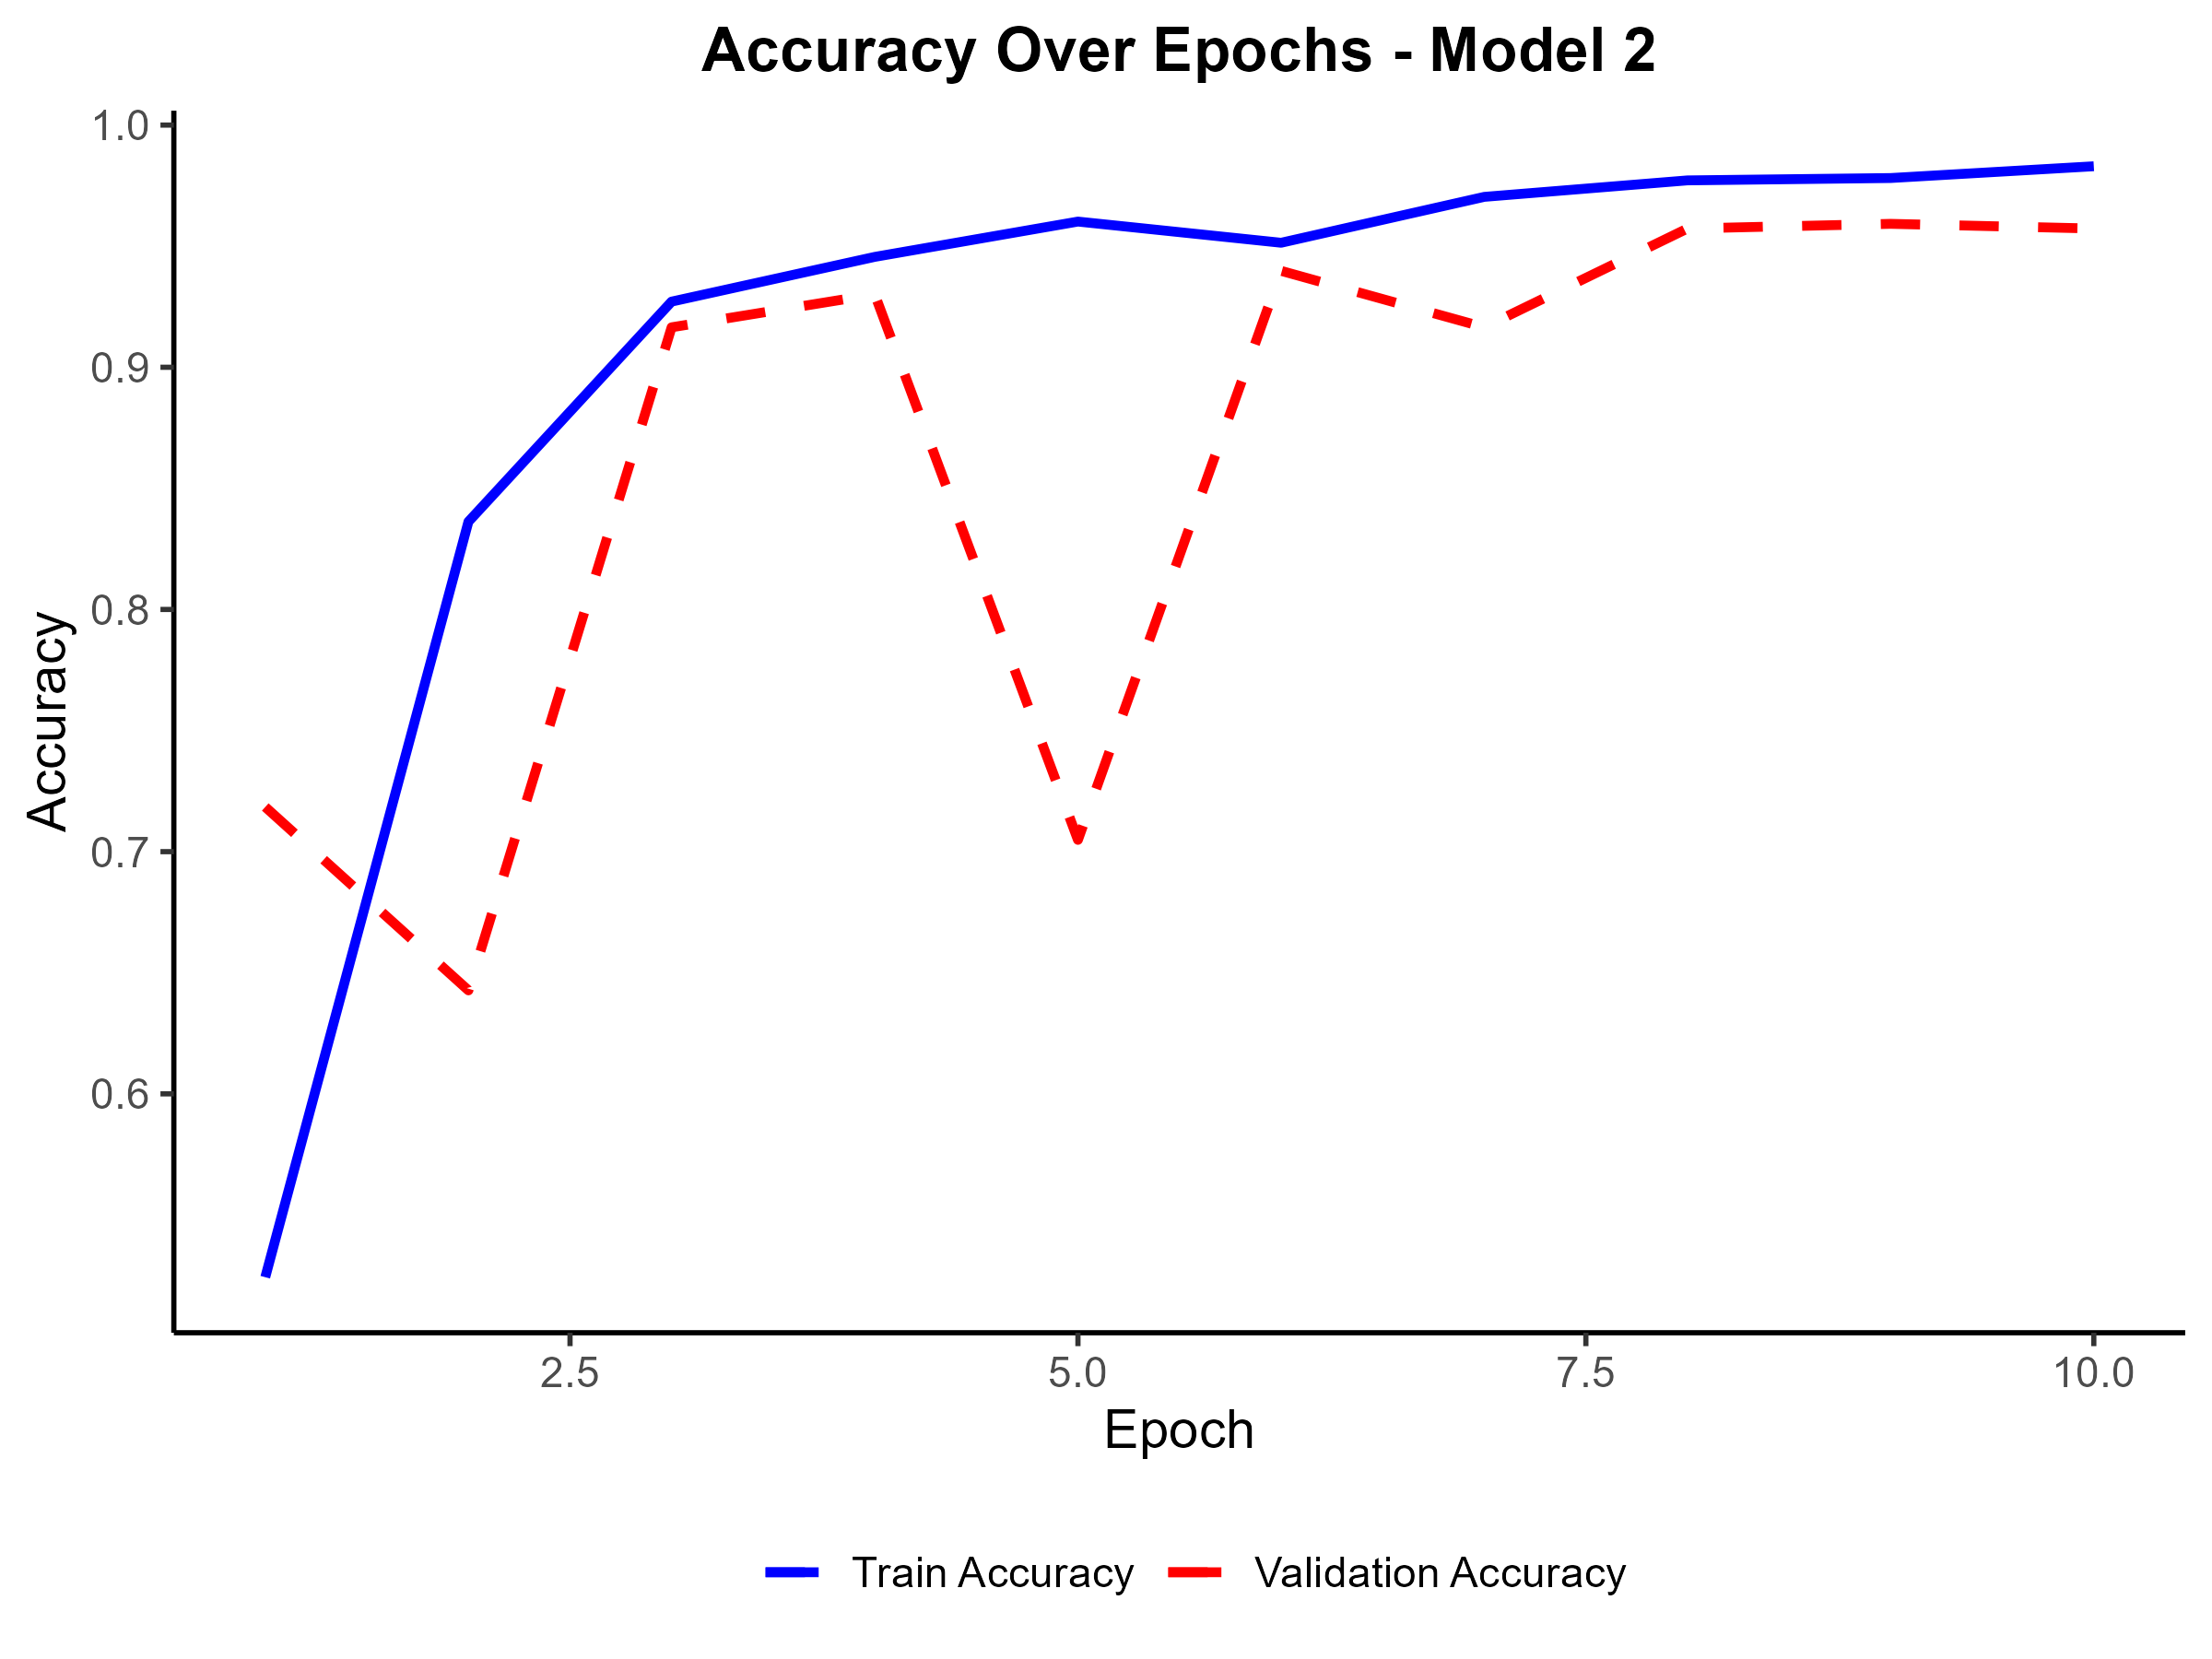
\includegraphics[width=0.8\linewidth]{results/accuracy_plot_model_2.png}
    \caption{Accuracy over epochs - Model 2 (Larger CNN).}
\end{figure}

\begin{figure}[H]
    \centering
    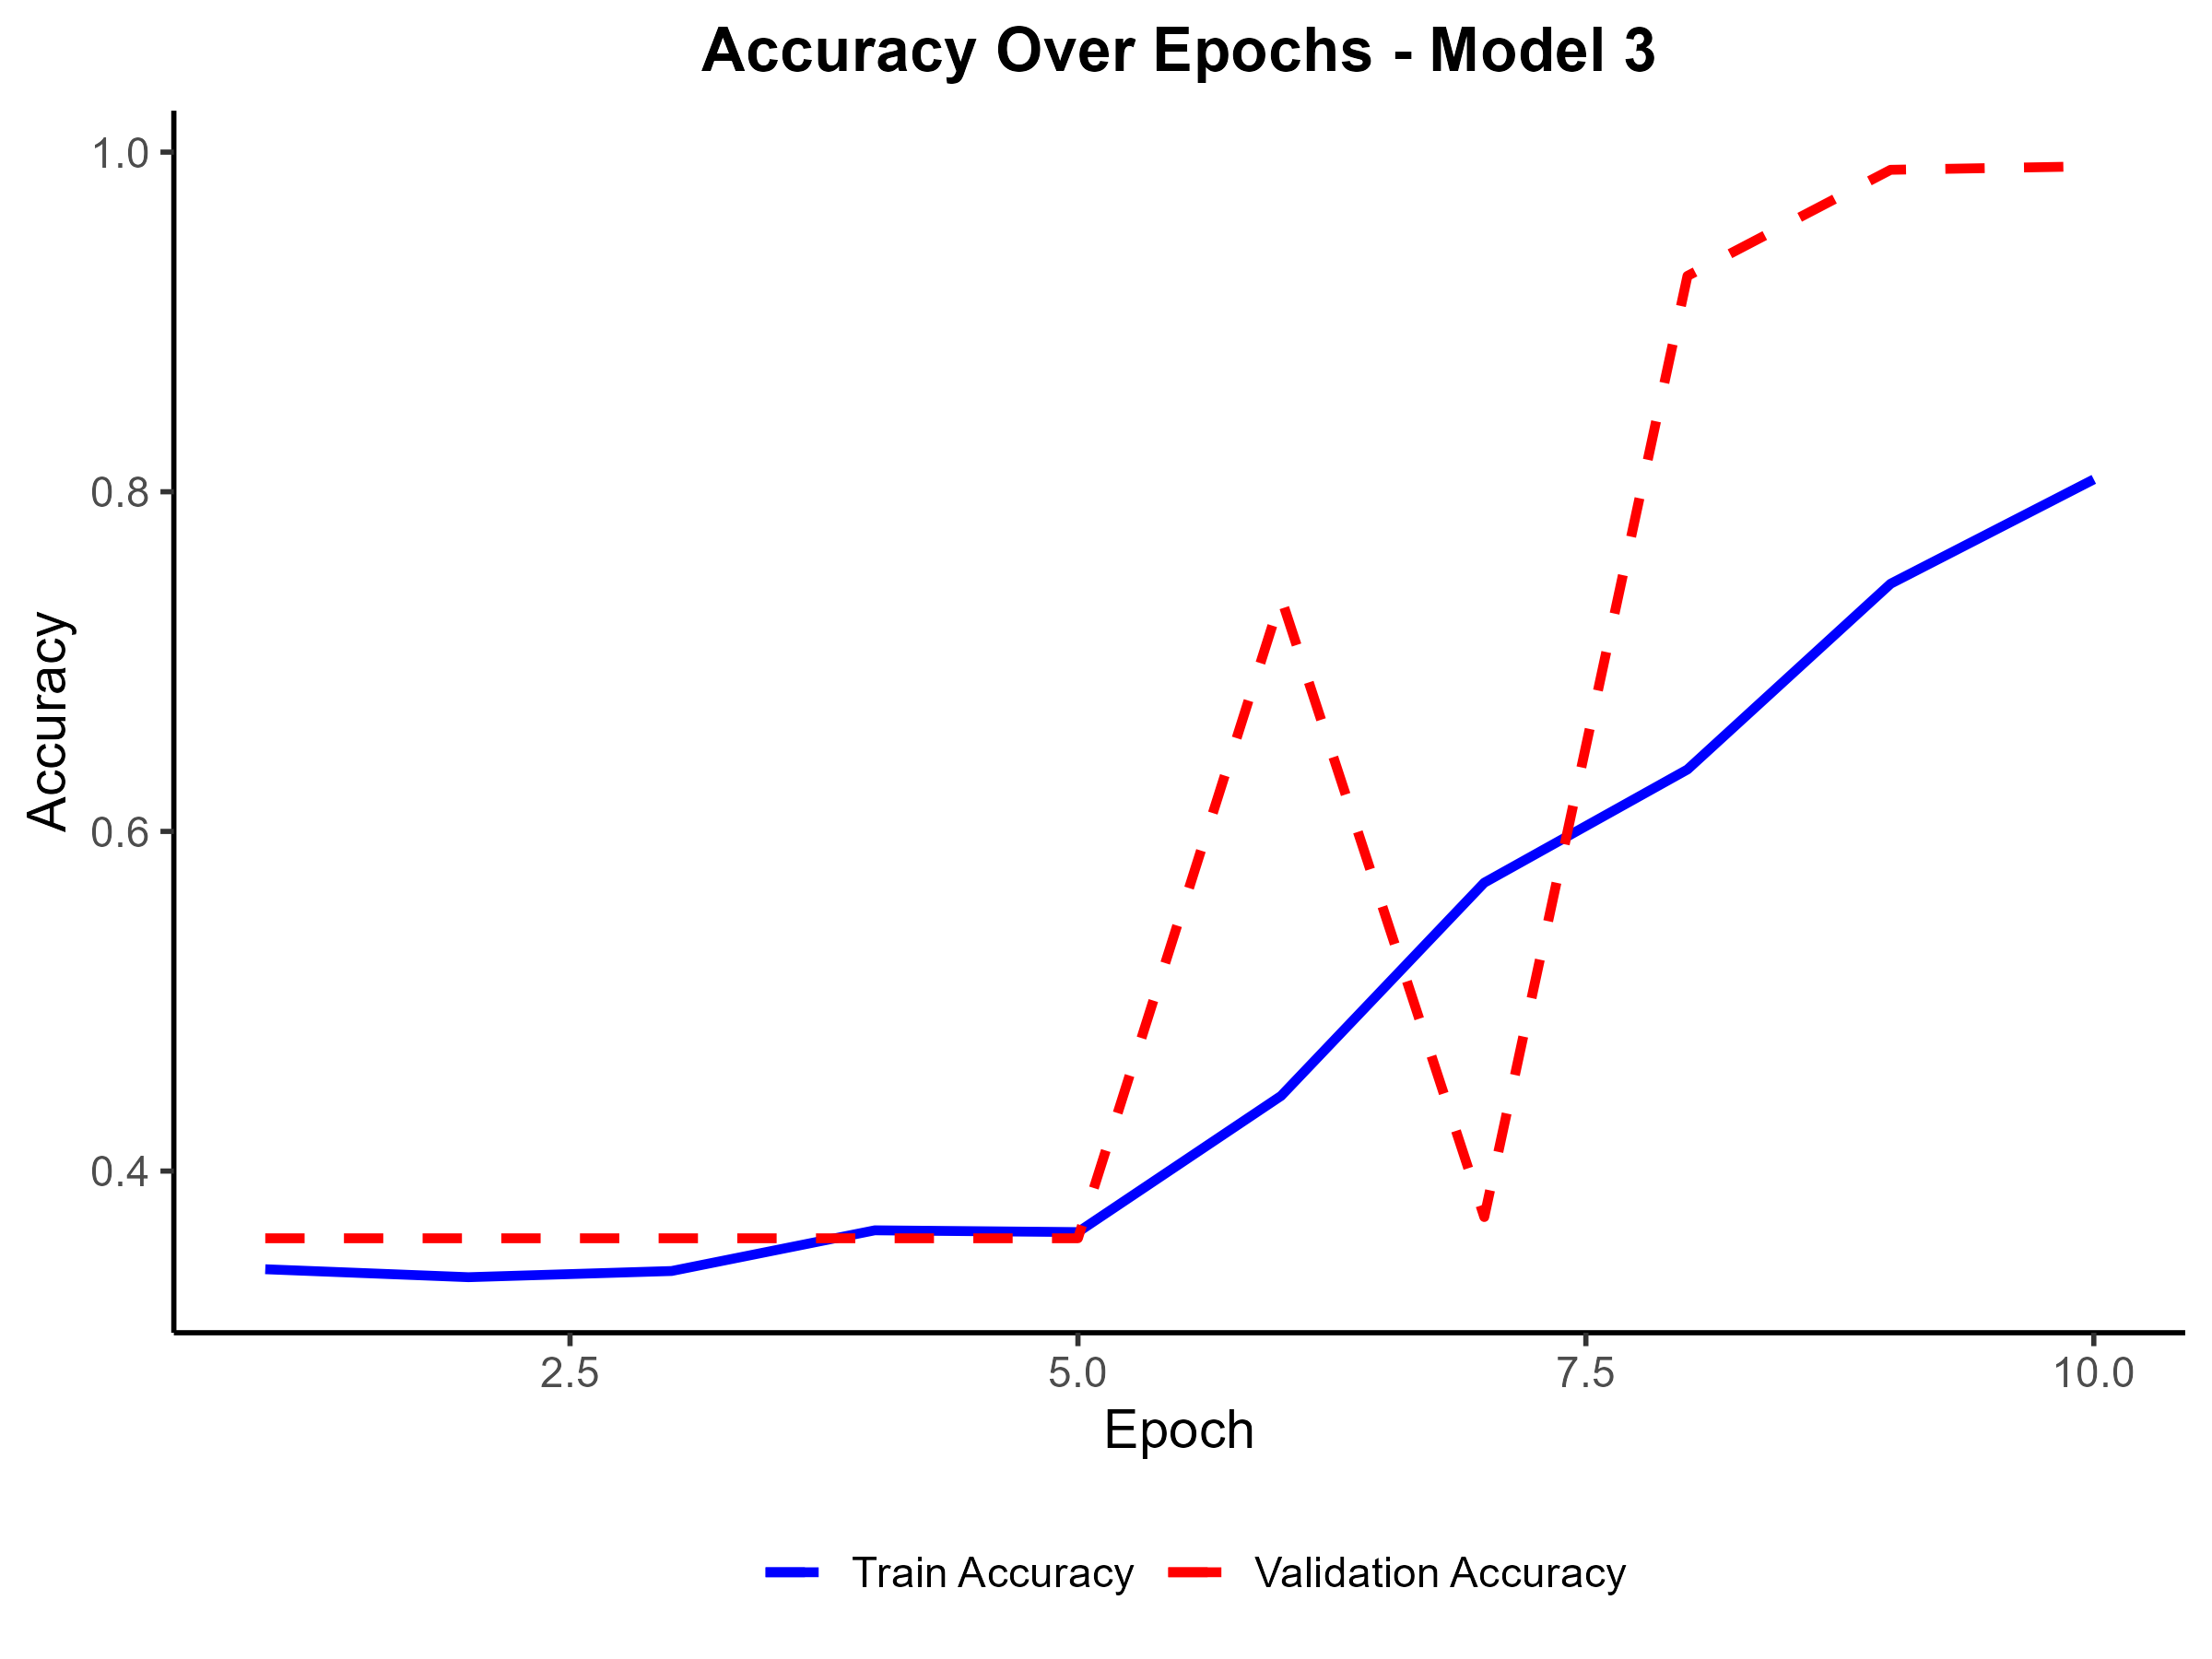
\includegraphics[width=0.8\linewidth]{results/accuracy_plot_model_3.png}
    \caption{Accuracy over epochs - Model 3 (CNN with Dropout).}
\end{figure}

\subsection{Model Test Accuracy}
The three convolutional neural network (CNN) models were evaluated on the test dataset. The accuracies for each model are as follows:

\begin{itemize}
    \item \textbf{Model 1 (Simple CNN)} achieved a test accuracy of \textbf{97.98\%}.
    \item \textbf{Model 2 (Larger CNN)} achieved a test accuracy of \textbf{95.65\%}.
    \item \textbf{Model 3 (CNN with Dropout)} achieved the highest test accuracy of \textbf{98.29\%}.
\end{itemize}

The results demonstrate that:
\begin{enumerate}
    \item Model 3, which included dropout layers to reduce overfitting, achieved the highest test accuracy. 
    \item Model 1, while simpler, performed exceptionally well, achieving a comparable accuracy of 97.98\%, suggesting that even a basic CNN can effectively classify images in this dataset.
    \item Model 2, despite having more layers, performed slightly worse than Model 1 and Model 3, with a test accuracy of 95.65\%. This indicates that increasing the complexity of the network does not always translate to better performance and may lead to overfitting.
\end{enumerate}


\subsection{Transfer Learning}
 I wanted to take the best performing model (Model 3 from above) and apply some transfer learning model on top to see if we can up the testing accuracy. I was already satisfied with Model 3's accuracy on a small subset of the data, thus this was just for curiosity. Transfer learning was applied using the MobileNetV2 architecture.

\begin{figure}[H]
    \centering
    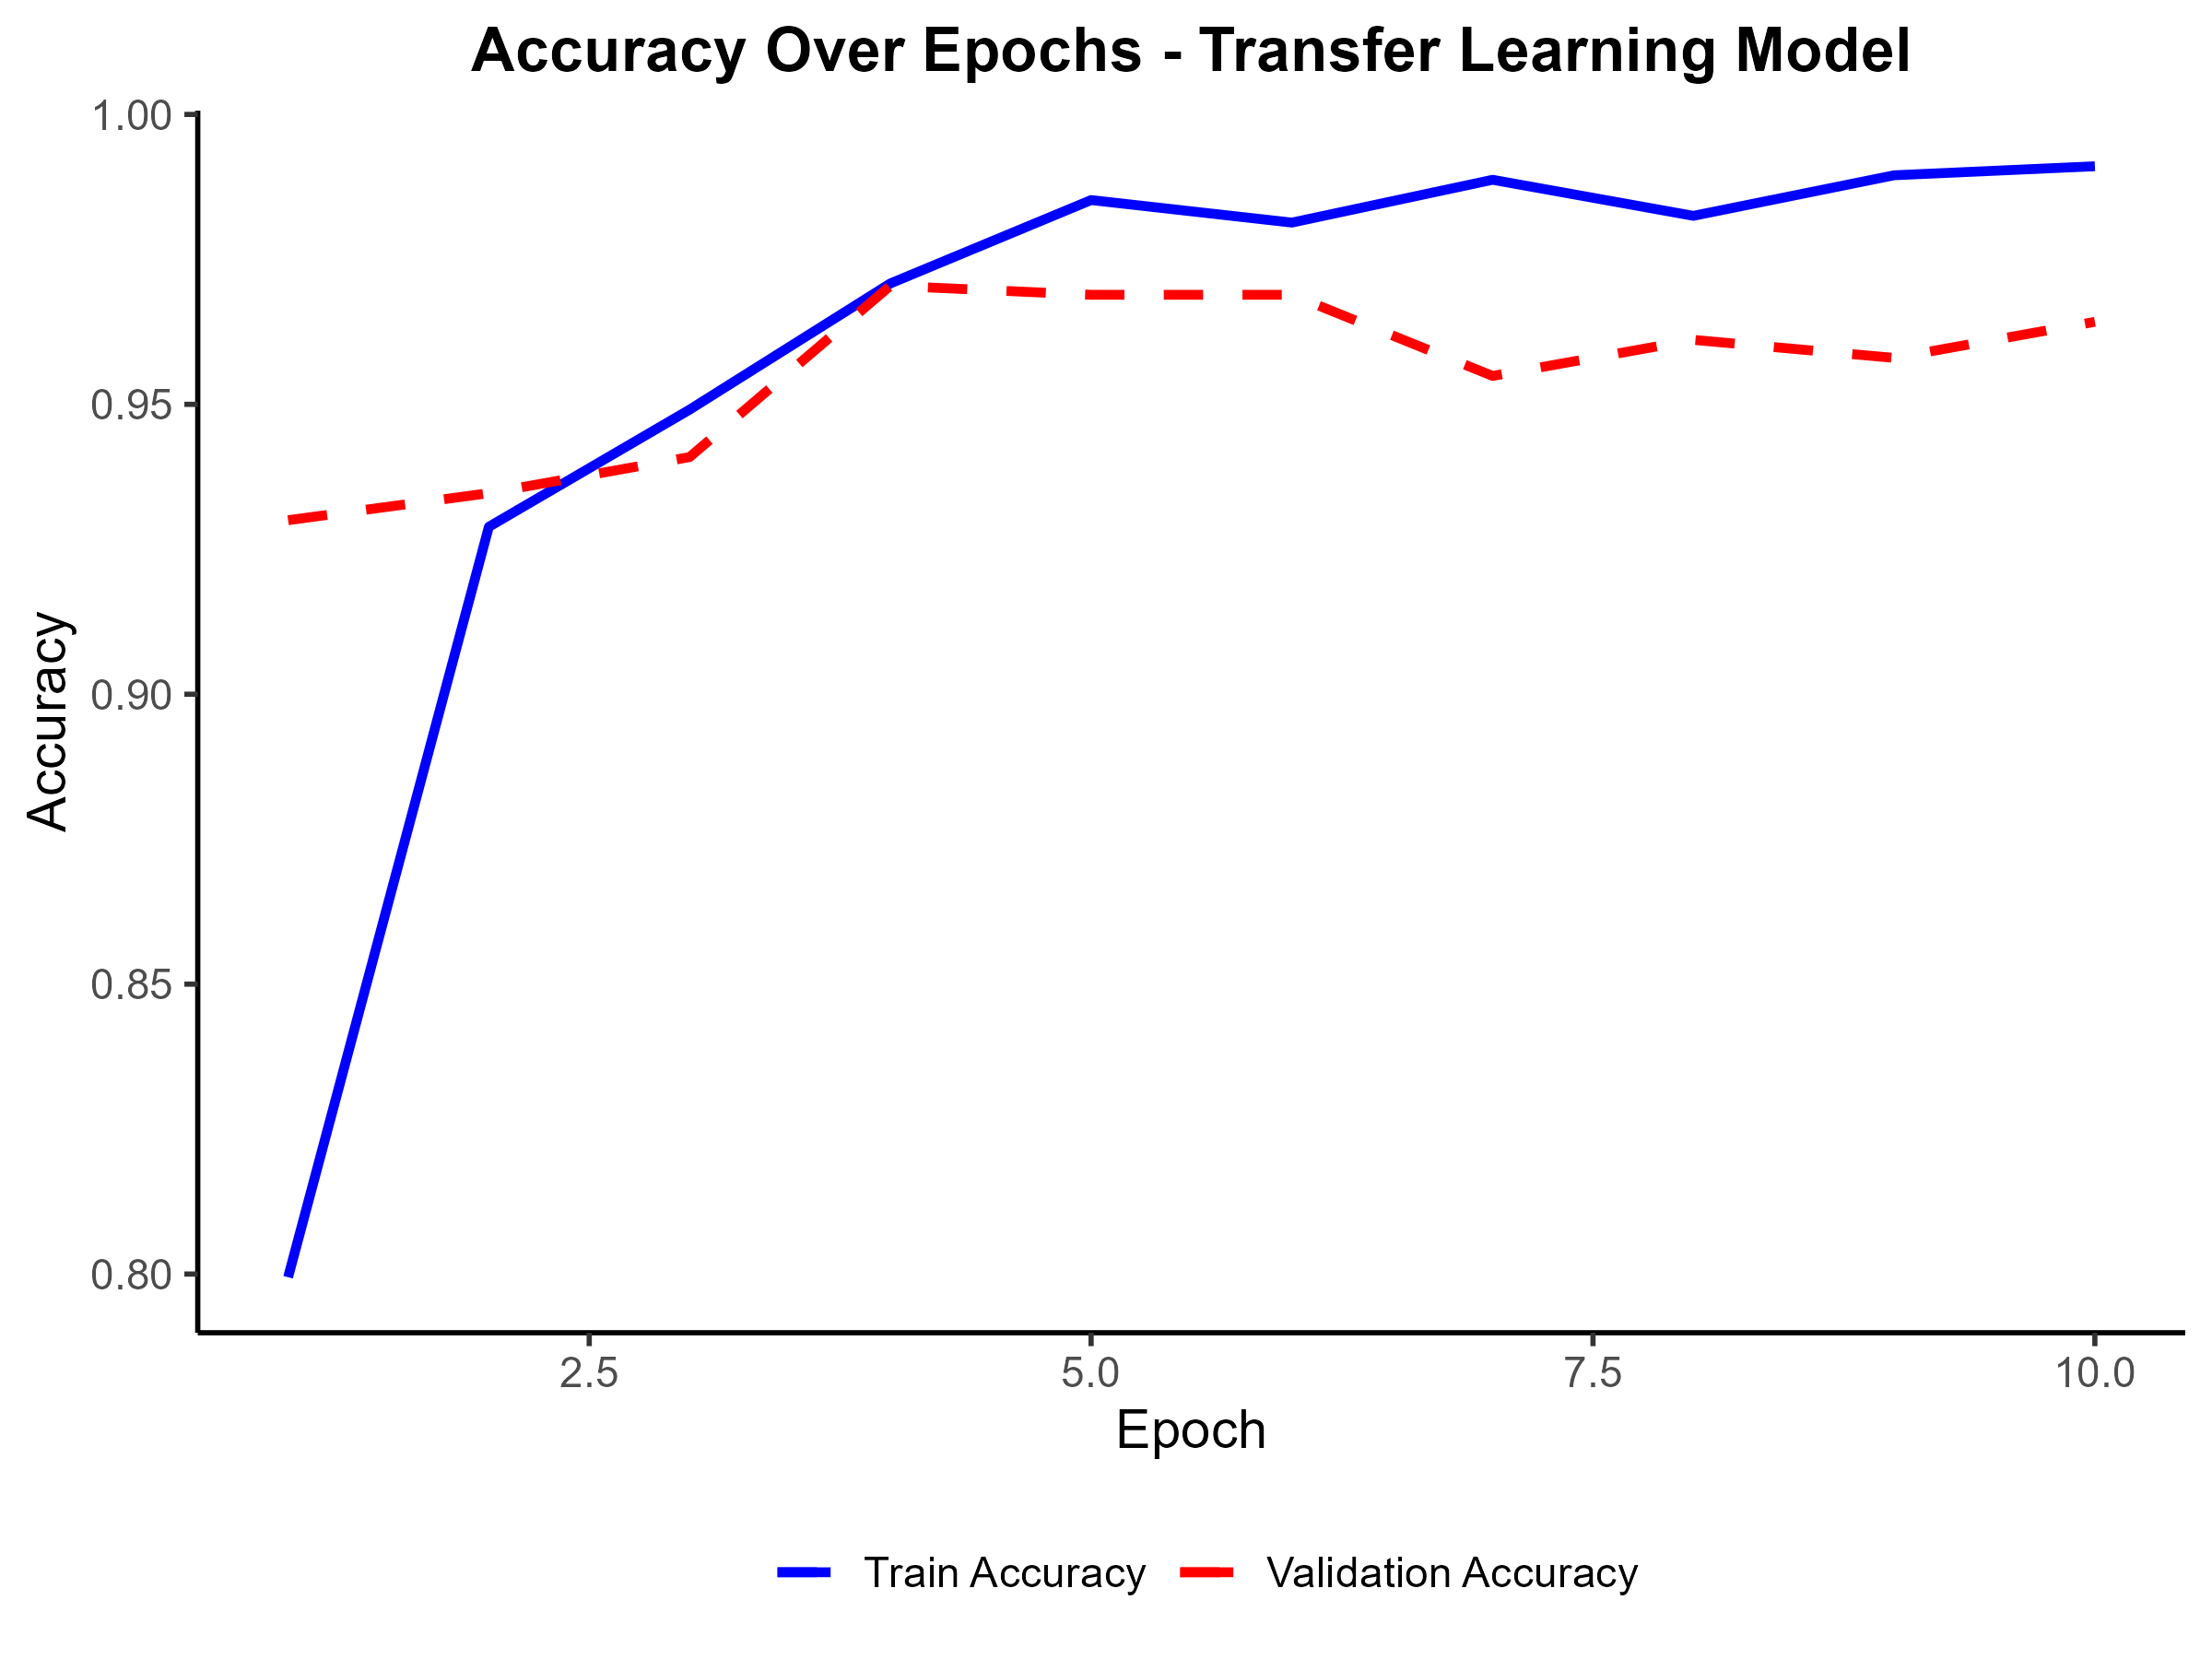
\includegraphics[width=0.8\linewidth]{results/accuracy_plot_transfer_model.png}
    \caption{Accuracy over epochs - Transfer Learning Model.}
\end{figure}

\begin{itemize}
    \item \textbf{Transfer Learning Model} achieved a test accuracy of \textbf{96.42\%}..
\end{itemize}


\section{Classification Results}
Both models performed well, but Model 3 suprisingly classified a few more photos correctly, making it the best model of the 4 tested with a 0.98 accuracy on the test dataset. In the misclassified images, you can see there are indeed a handful of testing images that the model got wrong. Some are hard to understand and it needs further investigation as to why they are misclassified. Others, like that of the incorrectly-classified birds actually appear in both the Transfer Model and Model 3, and are likely an artifact of decreasing the resolution of the images and thus the bird tail appears blurry and looks like a raccoon hand. 


\subsection{Classification Statistics}
The classification statistics for the transfer learning model are as follows:
\begin{itemize}
    \item \textbf{Number of correctly classified images}: 620
    \item \textbf{Number of misclassified images}: 23
\end{itemize}

The classification statistics for the best-performing model are as follows:
\begin{itemize}
    \item \textbf{Number of correctly classified images}: 632
    \item \textbf{Number of misclassified images}: 11
\end{itemize}


\subsection{Correctly Classified Images}

\begin{figure}[H]
    \centering
    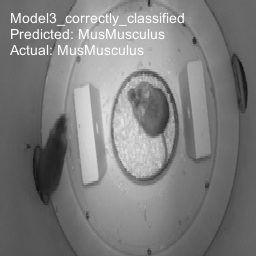
\includegraphics[width=0.3\linewidth]{results/Model3_correctly_classified_image_503.png}
    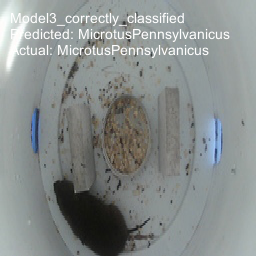
\includegraphics[width=0.3\linewidth]{results/Model3_correctly_classified_image_4.png}
    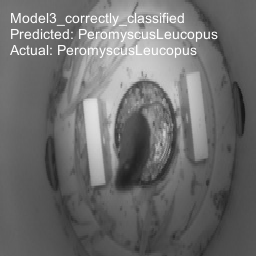
\includegraphics[width=0.3\linewidth]{results/Model3_correctly_classified_image_3.png}
    \caption{Examples of correctly classified image for Model 3.}
\end{figure}

\begin{figure}[H]
    \centering
    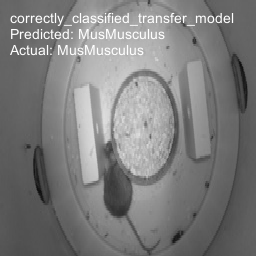
\includegraphics[width=0.3\linewidth]{results/correctly_classified_transfer_model_image_260.png}
    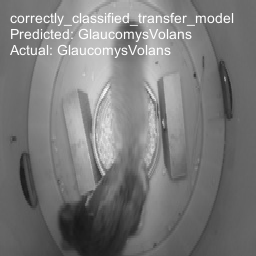
\includegraphics[width=0.3\linewidth]{results/correctly_classified_transfer_model_image_81.png}
    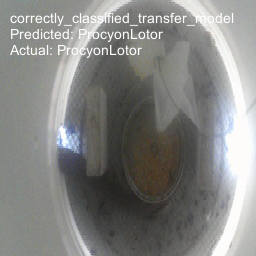
\includegraphics[width=0.3\linewidth]{results/correctly_classified_transfer_model_image_1.png}
    \caption{Examples of correctly classified image for the Transfer Model.}
\end{figure}

\subsection{Misclassified Images}

\begin{figure}[H]
    \centering
    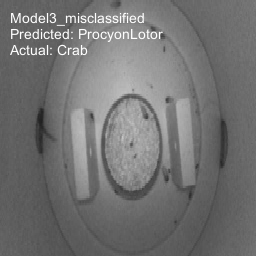
\includegraphics[width=0.3\linewidth]{results/Model3_misclassified_image_51.png}
    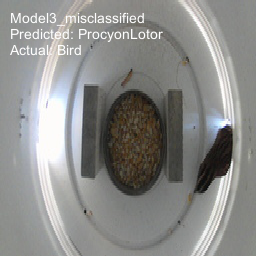
\includegraphics[width=0.3\linewidth]{results/Model3_misclassified_image_82.png}
    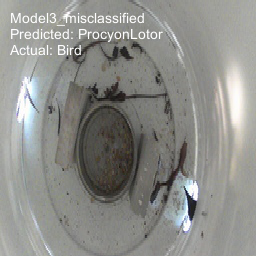
\includegraphics[width=0.3\linewidth]{results/Model3_misclassified_image_158.png}
    \caption{Examples of misclassified images for Model 3.}
\end{figure}

\begin{figure}[H]
    \centering
    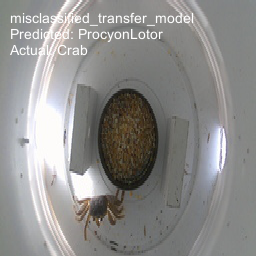
\includegraphics[width=0.3\linewidth]{results/misclassified_transfer_model_image_33.png}
    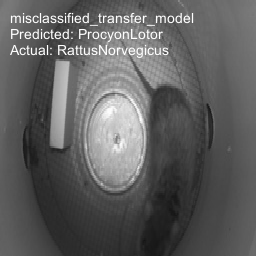
\includegraphics[width=0.3\linewidth]{results/misclassified_transfer_model_image_26.png}
    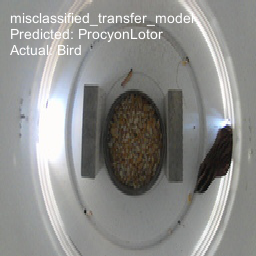
\includegraphics[width=0.3\linewidth]{results/misclassified_transfer_model_image_82.png}
    \caption{Examples of misclassified images for Transfer Model.}
\end{figure}


\section{Conclusion}
Overall, I am impressed by this model's performance. I really like how well it turned out, and will likely want to try this on one of the PC Towers at the BI (perhaps before sending it off to Dr. Porter.) I also would like to figure out a way to save the model as an R object to send to Dr. Porter, but perhaps it would be best for him to run the preprocessing scripts first to ensure his data is ina format for keras. Either way, I see this as a success!


\end{document}
